\section*{Zielsetzung}
Der Versuch soll überprüfen, ob die Dulong-Peptitsche Gesetz
angesprochenen Oszillation der Atome. Einer klassischen Beschreibung genügt,
oder ob eine quantenmechanische Beschreibung von Nöten ist.


\section{Theorie}

\subsection{Definition der spezifischen Wärmekapazität}

Findet an einem Körper eine Temperaturänderung $\Delta T$ statt, ohne das an ihm 
Arbeit verrichtet wird. So kommt es zu einer Wärmeaufnahme bzw. Abgabe $\Delta Q$.
Mit dem ersten Hauptsatz der Thermodynamik ergibt sich dann der Zusammenhang

\begin{equation*}
\Delta Q=m c \Delta T.
\end{equation*}

Dabei sei $m$ die Masse und $c$ die Wärmekapazität 
des Körpers.
Wird zusätzlich die Masseneinheit berücksichtig,
so wird $c$ als spezifische Wärmekapazität bezeichnet.

Des Weiteren gibt die Molwärme $C$
an, was für eine Wärmemenge $\map{d}Q$ benötigt wird,
um ein Mol eines Stoffes um $\map{d}T$ zu erwärmen.

Dabei hängt der Betrag der Molwärme davon ab, unter welchen Bedingungen 
die Temperaturänderung hervor gerufen wird.
Hierbei wird zwischen der spezifischen Wärmekapazität bei konstantem
Volumen $C_{V}$ und bei konstantem Druck $C_{p}$ unterschieden.
Die Größe $C_{V}$ sei gegeben durch:

\begin{equation}
\label{eq:molwarme}
C_V=\left(\frac{\map{d}U}{\map{d}T}\right)_V
\end{equation}


\subsection{Dulong-Petitsch-Gesetz}

Das Dulong-Petitsche-Gesetz sagt aus, dass die Atomwärme (im festem Aggregatzustand) bei 
konstantem Volumen unabhängig von den chemischen Eigenschaften eines Elementes 
und gleich $3R$ sei.
Man bezeichnet $R$ als die allgemeine Gaskonstante.
Das Gesetz begründet die makroskopischen thermodynamischen Phänomene 
auf zufällige mikroskopischen Bewegungen der Atome.
Das Dulong-Petitsch-Gesetz wird zum Teil aus dem 
das sogenannte Äquipartitionstheorem hergeleitet. 
Das Theorem gibt Rückschlüsse auf die kinetische Energie eines Atomes
im thermischen Gleichgewicht, durch:

\begin{equation*}
\left< E_{kin} \right>=\frac{1}{2}kT
\end{equation*} 

Mit diesem und weitern Zusammenhängen folgt für die innere Energie $U$ 
einer Gitterstruktur mit drei Freiheitsgraden:

\begin{equation*}
\left< U_{fest} \right> = 3 \left< U \right>=3RT \quad \Rightarrow \quad C_{V}\overset{\eqref{eq:molwarme}}{=}3R
\end{equation*}

\subsubsection{Quantenmechanische Betrachtung}
Bei der quantenmechanischen Betrachtung wird angenommen, 
dass die oszillierenden Atome nur quantisierte Energiezustände $\Delta u=n\hbar \omega \quad n\in\mathbb{N}$
annehmen können.
Mit Zuhilfenahme der Boltzmann-Verteilung kann dann auf den Zusammenhang 
\begin{equation}
\label{eq:quant}
\left< U_{qm} \right> =\frac{3N_L \hbar \omega}{\exp\left(\hbar \frac{\omega}{k} T\right) -1}
\end{equation}

geschlossen werden. Dieser gilt für Bewegungen mit drei Freiheitsgraden.
Die Konstante $N_L = \SI{6.02e23}{\per\mol}$ wird als Loschmidtsche Zahl bezeichnet.
Für $T\to\infty$ läuft \eqref{eq:quant} gegen, den aus der klassischen Physik bekannten Wert, 
$3RT$.

\subsection{Bestimmung der spezifischen Wärmekapazität}
Da eine experimentelle Bestimmung der spezifischen Wärmekapazität 
bei konstanten Volumen $C_V$ kaum möglich ist.
Bestimmt stattdessen die Wärmekapazität bei konstanten Druck $C_P$.
Beide Größen könnenen durch den Zusammenhang

\begin{equation}
\label{eq:umrechnung_cp_cv}
C_P-C_V=9\alpha^2\kappa V_0 T \quad \text{mit} \kappa=V\left(\frac{\partial p}{\partial V}\right)_T
\end{equation}

ineinander umgerechnet werden.
Hierbei sei $\alpha$ ein linearer Ausdehnungskoeffizient, $\kappa$ das Kompressionsmodul und
$V_0$ das Molvolumen.

Die Bestimmung erfolgt mithilfe eines Kalorimeters,
eins rohrförmigen Probekörpers mit der Masse $m_k$ und der Temperatur 
$T_k$. Zusätzlich gibt es ein mit Wasser gefülltes Gefäß.
Das Wasser besitzt die Masse $m_w$ und die Temperatur $T_w$.
Nach Eintauchen des Körpers stellt sich im Gefäß die 
Mischtemperatur $T_w$ ein. 
Es ergibt sich folgende Abhängigkeit:

\begin{equation*}
\label{eq:zusammenhang_ck}
c_k=\frac{\left(c_wm_w+c_gm_g\right)\left(T_m-T_w\right)}{m_k\left(T_k-T_m\right)}
\end{equation*}

Die Wärmekapazität des Kaloriemeters wird druch $c_gm_g$ dargestellt.
In in einer weitern Messung wird diese bestimmt.
Bei dieser werden zwei Wassermengen mit $m_x$ und $m_y$ und den 
dazugehörigen Temperaturen $T_x$ und $T_y$ miteinander vermischt.
Mit der sich einstellenden Temperatur $T_M$ kann dann
durch den Zusammenhang:
\begin{equation}
\label{eq:zusammenhang_cgmg}
c_gm_g=\frac{c_wc_y\left(T_y-T_M\right)-c_wm_x\left(T_M-T_x\right)}{\left(T_M-T_x\right)}
\end{equation}
auf die Wärmekapazität geschlossen werden.

\subsection{Thermoelemente und ihre Funktionsweise} %Skizze
\begin{figure}
  \centering
  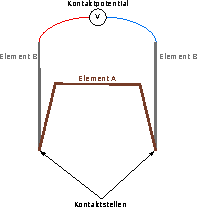
\includegraphics[width=0.45\textwidth]{bilder/thermoelement.pdf}
  \caption{Schematische Darstellung eines Thermoelements}
  \label{fig:thermo}
\end{figure}
Ein schematischer Aufbau eines Thermoelements ist in Abbildung \ref{fig:thermo}
zu erkennen.
Ein Thermoelement wird dazu genutzt, um eine sich schnell ändernde 
Temperatur zu messen. 
Denn es zeichnet sich durch seine hohe Einstellungsgeschwindigkeit aus.
Es besteht aus zwei Metallen, die sich jeweils durch
verschiedene Wärmeleitkoeffizienten auszeichnen.
Am Ende des Thermoelementes befindet sich ein Punkt an dem sich
beide Elemente berühren. Dieser Punkt wird als Berührungspunkt 
bezeichnet.
Ein Thermoelement besitzt zwei Berührungsstellen.
Diese messen jeweils unterschiedliche Temperaturen $T_1$ und $T_2$.
Herrscht eine Temperaturdifferenz zwischen $T_1$ und $T_2$, so 
stellt sich zwischen den Kontaktstellen ein Kontaktpotenzial 
ein. 
Durch Messung der Spannung kann anschließend auf 
Temperaturdiffere	nz geschlossen werden.







